\section{Diseño de simulación para compresión sin pérdida en simuladores tipo Schrödinger}
\label{sec:simulation-design}

Una vez seleccionado el simulador base y definida la biblioteca de compresión a emplear, el siguiente paso consiste en establecer una arquitectura
de simulación que permita introducir compresión sin pérdida sin alterar la semántica del simulador de estado completo. En esta sección se presenta
una propuesta de diseño en niveles de abstracción, pensada para ser reutilizable en cualquier simulador tipo Schrödinger cuyo estado cuántico se
represente como un vector de amplitudes complejas en doble precisión.

\begin{figure}[H]
    \centering
    \caption{Arquitectura abstracta para integración de compresión sin pérdida en simuladores tipo Schrödinger}
    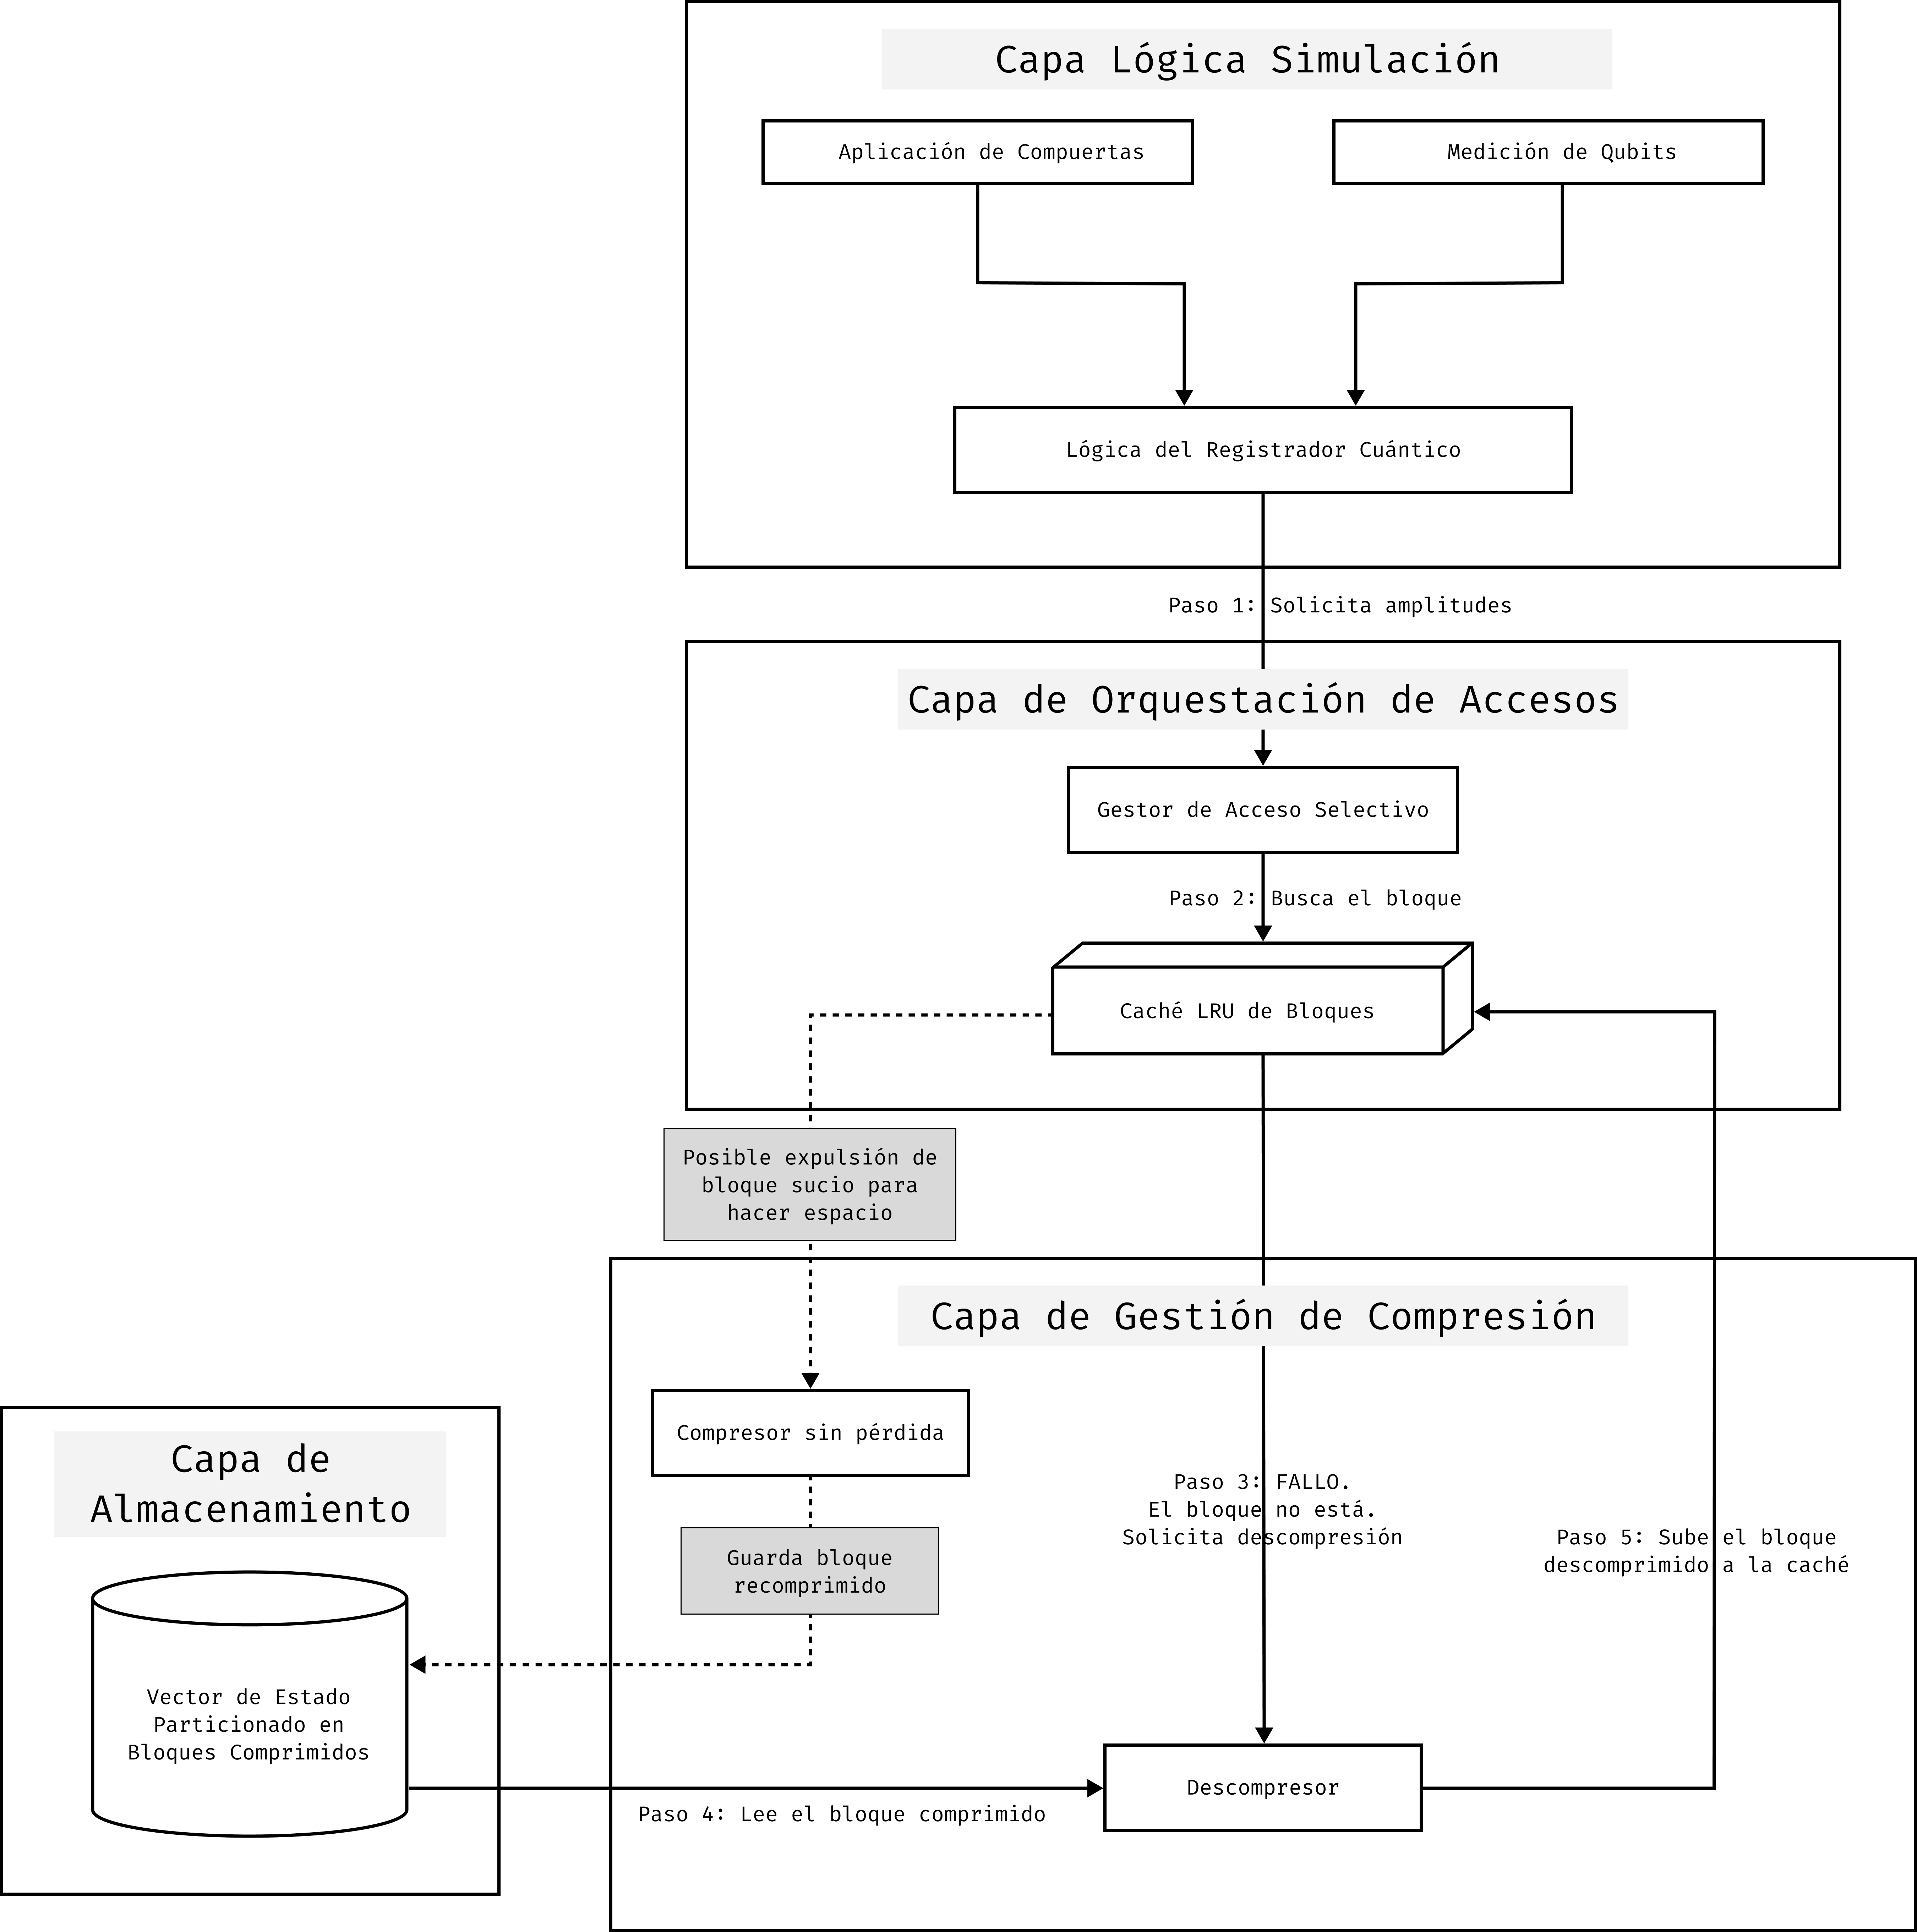
\includegraphics[width=0.5\linewidth]{images/simulation-design-architecture}
    \label{fig:simulation-design-architecture}
\end{figure}

\subsection{Objetivos del diseño}

El diseño propuesto busca satisfacer cuatro objetivos simultáneos. En primer lugar, reducir la huella de memoria del vector de estado, que crece
exponencialmente con el número de qubits. En segundo lugar, preservar la exactitud numérica del simulador, evitando pérdidas de precisión en las
amplitudes complejas. En tercer lugar, impedir que cada compuerta obligue a reconstruir el vector de estado completo en memoria densa. Finalmente,
se requiere que la sobrecarga temporal introducida por la compresión permanezca controlada y pueda ser ajustada mediante parámetros de diseño.

Estos objetivos conducen a una separación clara entre la lógica del simulador y la estrategia de almacenamiento. La lógica cuántica continúa
operando sobre amplitudes complejas, compuertas y mediciones, mientras que la representación física del vector puede variar entre una forma densa
y una forma comprimida por bloques, siempre que ambas expongan el mismo comportamiento observable.

\subsection{Representación por bloques del vector de estado}

La decisión estructural principal consiste en particionar el vector de estado en bloques independientes de tamaño fijo. Cada bloque agrupa un número
determinado de estados base consecutivos y almacena sus partes real e imaginaria como un arreglo contiguo de números en punto flotante. Esta
organización convierte el problema global de compresión del estado completo en una colección de problemas locales sobre subarreglos más pequeños.

La ventaja de esta representación es doble. Por una parte, cada bloque puede comprimirse y descomprimirse sin depender del contenido de los demás,
lo que facilita actualizaciones localizadas. Por otra, el tamaño del bloque se convierte en un parámetro de diseño que permite balancear dos efectos
opuestos: bloques más grandes tienden a favorecer el ratio de compresión, mientras que bloques más pequeños reducen el costo de acceso cuando solo
una fracción del vector es requerida.

\begin{figure}[H]
    \centering
    \caption{Particionamiento abstracto del vector de estado en bloques independientes}
    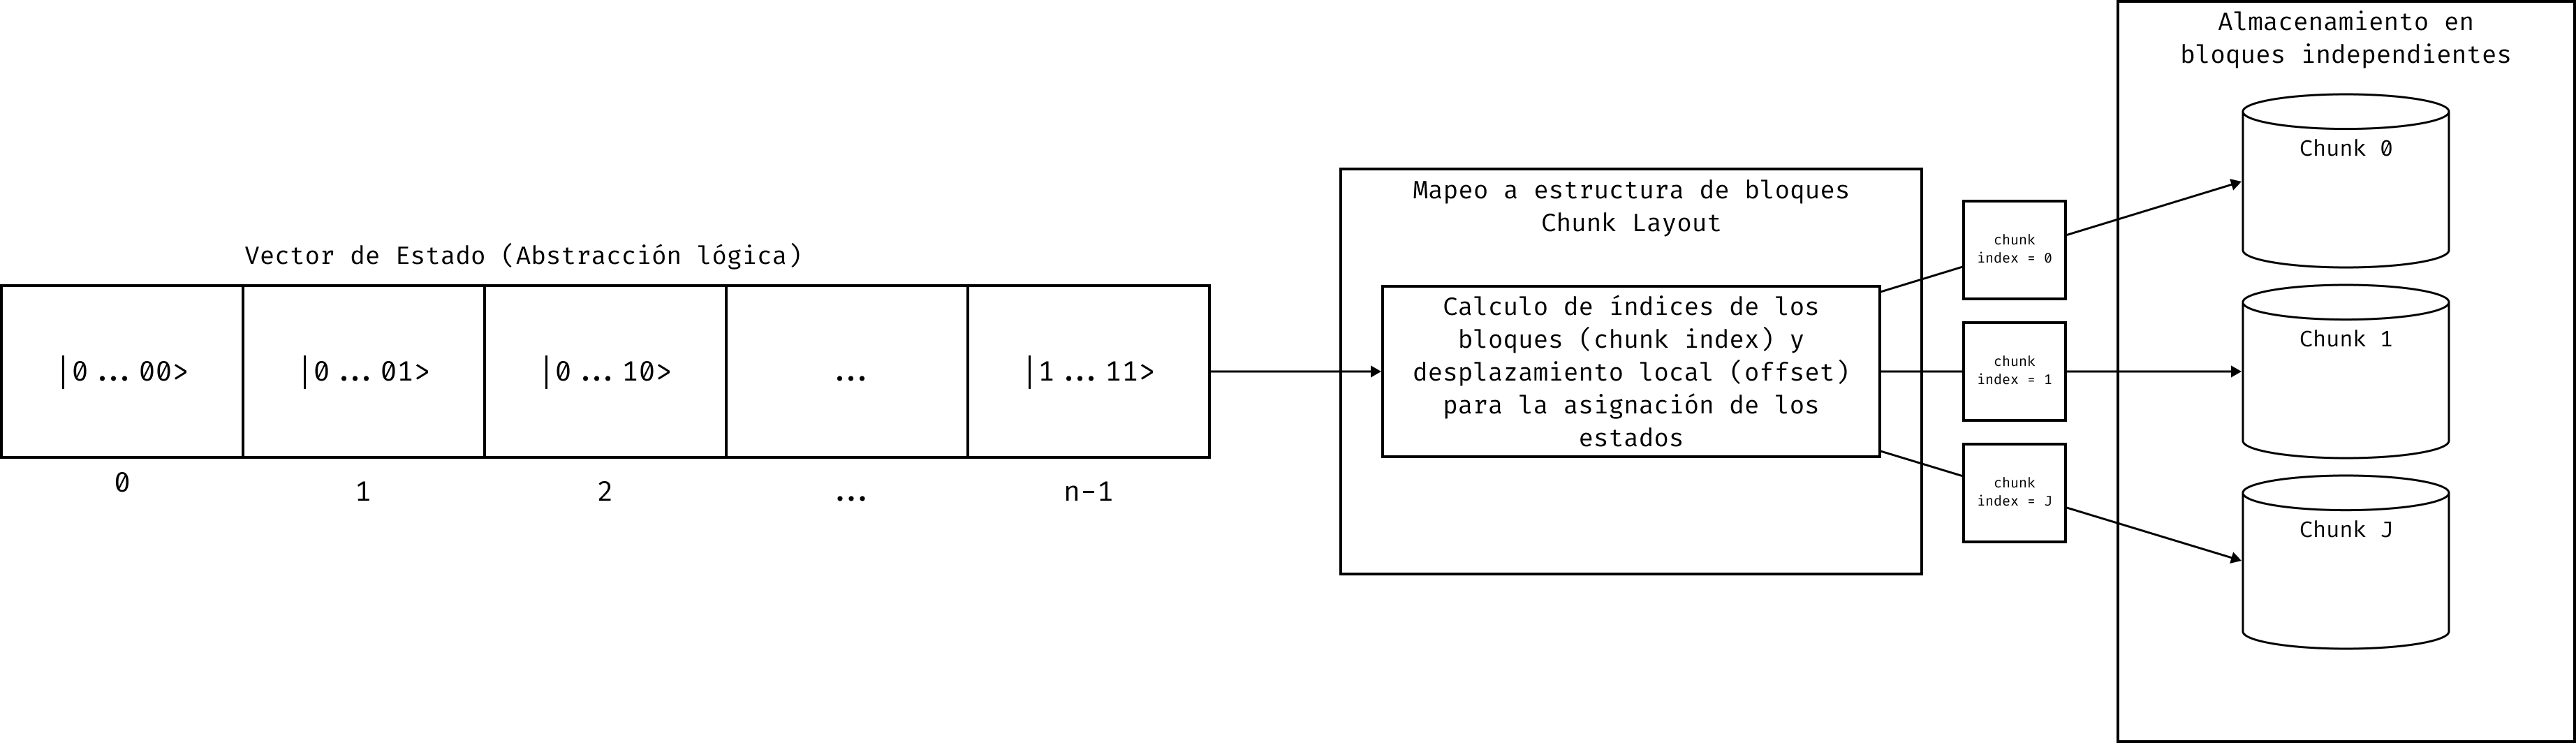
\includegraphics[width=1\linewidth]{images/simulation-design-blocks}
    \label{fig:simulation-design-blocks}
\end{figure}

\subsection{Descompresión selectiva y estrategia de acceso}

En una arquitectura densa tradicional, cualquier compuerta opera directamente sobre el arreglo completo de amplitudes. En contraste, cuando el
estado está comprimido por bloques, la política de acceso debe asegurar que solo se materialicen en memoria densa los bloques realmente tocados por
la operación actual. De este modo, una compuerta de uno o dos qubits no desencadena una descompresión global, sino un proceso local de adquisición
de bloques, modificación y posterior recompresión.

Esta idea conduce a una estrategia de descompresión selectiva. Cada acceso a una amplitud o a un conjunto de amplitudes se traduce en la identificación
de los bloques involucrados. Si un bloque ya se encuentra disponible en forma descomprimida, la operación se realiza directamente sobre ese buffer.
Si el bloque aún está almacenado en forma comprimida, primero se descomprime, se ejecuta la actualización necesaria y luego se conserva temporalmente
en memoria de trabajo para evitar recomprimirlo de inmediato si es probable que vuelva a usarse en operaciones posteriores.

Desde el punto de vista algorítmico, esta estrategia es especialmente relevante para compuertas que inducen accesos repetidos a subconjuntos del
estado, así como para secuencias cortas de compuertas sobre qubits cercanos. En esos casos, mantener un subconjunto pequeño del vector en memoria
descomprimida puede amortiguar el costo de las transiciones entre representación comprimida y representación densa.

\subsection{Caché LRU de bloques descomprimidos}

Para sostener la estrategia anterior se introduce una caché de bloques descomprimidos. Su función es actuar como un conjunto de trabajo temporal
que almacena los bloques accedidos recientemente. Cuando una operación necesita un bloque, primero consulta la caché. Si el bloque está presente,
ocurre un acierto y se evita una nueva descompresión. Si el bloque no está presente, ocurre un fallo, el bloque se recupera desde almacenamiento
comprimido y se incorpora al conjunto de trabajo.

La política de reemplazo adoptada es del tipo \emph{Least Recently Used} (LRU). Bajo esta política, cuando la caché está llena y se necesita espacio
para un nuevo bloque, se expulsa el bloque cuyo último acceso sea el más antiguo. La elección de LRU es adecuada para este contexto porque muchas
secuencias de compuertas presentan localidad temporal: un bloque recién usado tiene mayor probabilidad de volver a ser requerido en el corto plazo
que uno accedido hace muchas operaciones.

Si el bloque expulsado fue modificado, debe recomprimirse antes de abandonar la caché. Si no fue modificado, puede descartarse sin costo de escritura.
Esta distinción entre bloques limpios y sucios evita recompresiones innecesarias y reduce la sobrecarga total del sistema.

\begin{figure}[H]
    \centering
    \caption{Esquema conceptual de la caché LRU de bloques descomprimidos}
    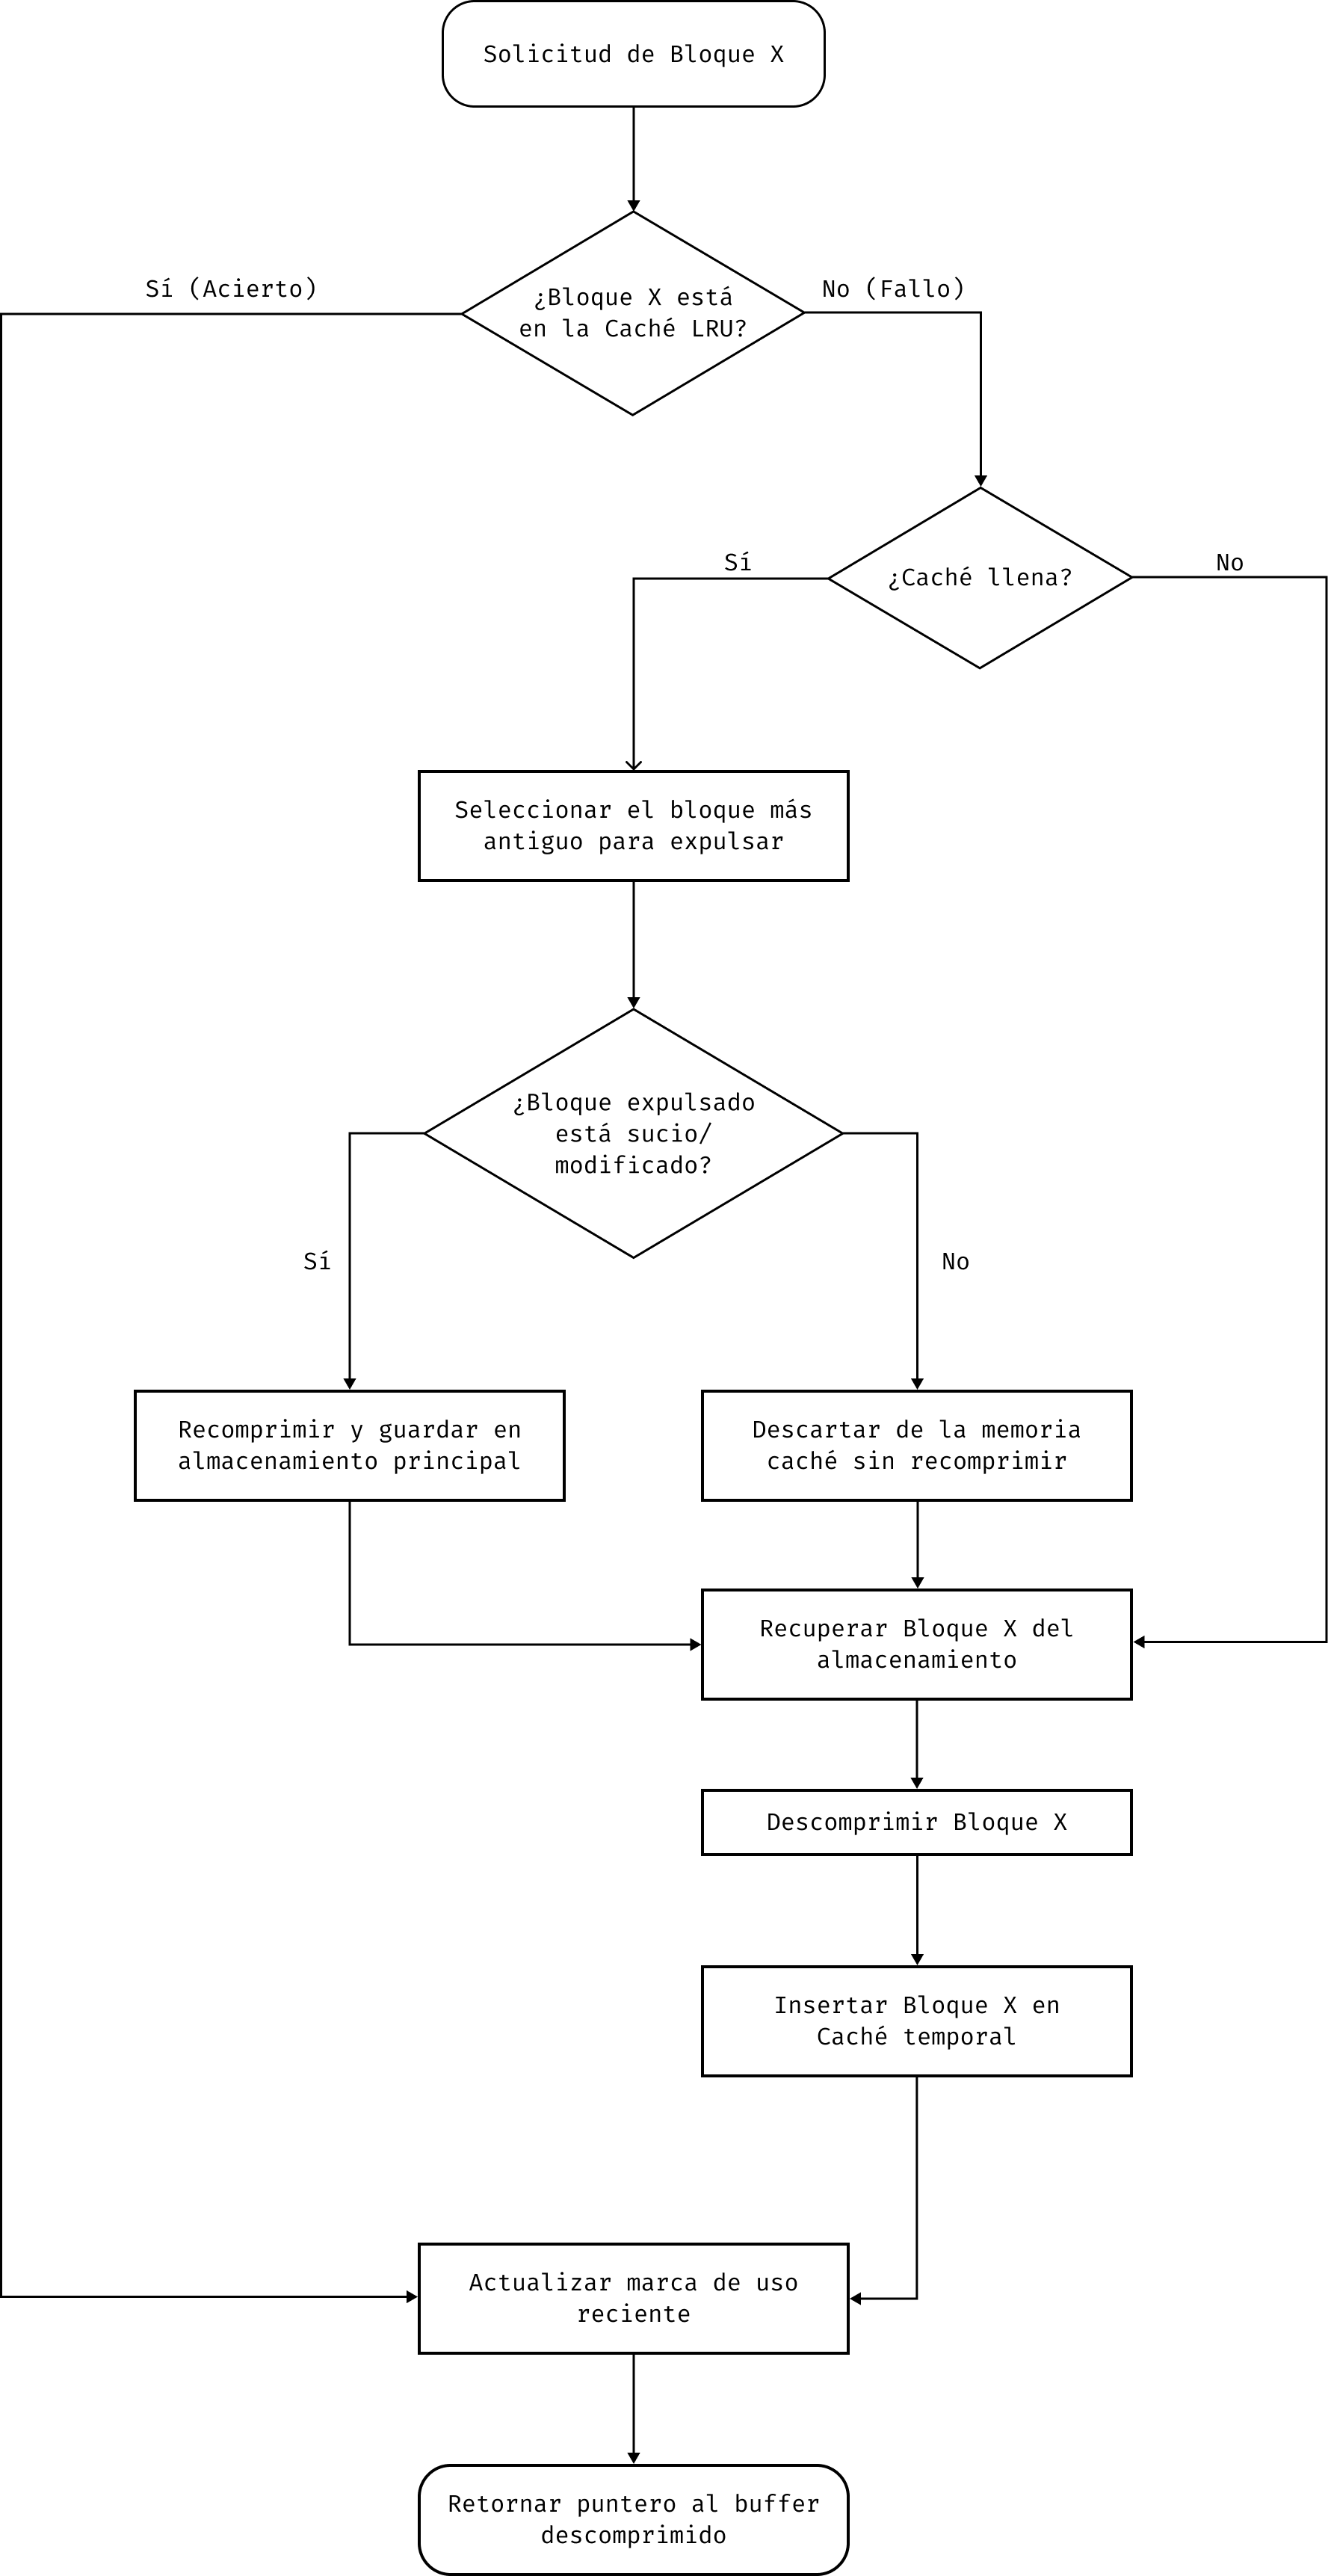
\includegraphics[height=0.6\textheight]{images/simulation-design-lru}
    \label{fig:simulation-design-lru}
\end{figure}

\subsection{Flujo de compresión y descompresión}

La compresión propuesta se entiende como un pipeline de etapas reversibles sobre cada bloque. Primero, el bloque en doble precisión se organiza como
un arreglo contiguo de valores. Luego puede aplicarse una transformación previa sobre la representación binaria de estos datos, por ejemplo una
variante de \emph{shuffle} o \emph{bitshuffle}, con el objetivo de exponer regularidades entre bytes o planos de bits. Finalmente, el flujo transformado
se entrega a un compresor sin pérdida de baja latencia.

El proceso inverso ocurre solo cuando el bloque es requerido por una operación. El bloque comprimido se descomprime, se invierte la transformación
previa y se obtiene nuevamente el arreglo denso de amplitudes listo para ser manipulado por la lógica del simulador. La clave del diseño es que esta
secuencia solo se ejecuta sobre los bloques activos y no sobre la totalidad del vector.

Para operaciones que afectan amplitudes pertenecientes a un mismo bloque, la actualización es enteramente local. Cuando la operación cruza bloques,
la arquitectura requiere adquirir simultáneamente los bloques involucrados, descomprimir ambos, ejecutar la actualización y decidir luego cuáles
mantener temporalmente en caché y cuáles devolver al almacenamiento comprimido. Este es el punto donde el tamaño de la caché y la granularidad de los
bloques influyen de manera más visible sobre el costo temporal.

\begin{figure}[H]
    \centering
    \fbox{\parbox{0.82\linewidth}{\centering
        Espacio reservado para una figura del flujo ``adquirir bloque -- descomprimir -- modificar -- marcar como sucio -- recomprimir'' y su variante
        para operaciones entre bloques distintos.}}
    \caption{Flujo abstracto de acceso y actualización de bloques comprimidos}
    \label{fig:simulation-design-flow}
\end{figure}

\subsection{Ventajas, parámetros y limitaciones del diseño}

El principal beneficio de esta arquitectura es que desacopla el ahorro de memoria de la necesidad de reconstruir por completo el vector de estado en
cada operación. Además, introduce parámetros claros y controlables: tamaño del bloque, número de entradas en caché, política de reemplazo y tipo de
compresor sin pérdida. Esto permite adaptar la arquitectura a diferentes patrones de acceso y a distintas disponibilidades de memoria.

No obstante, la arquitectura también presenta limitaciones. Si los estados cuánticos generados por el algoritmo son poco compresibles, la reducción
de memoria puede resultar modesta. Del mismo modo, si las compuertas inducen accesos dispersos sobre muchos bloques distintos, la tasa de fallos de
caché puede crecer y aumentar la cantidad de descompresiones. Por esta razón, el análisis experimental posterior debe estudiar el compromiso entre
ratio de compresión, latencia y tamaño del conjunto de trabajo.

En conjunto, los elementos anteriores delimitan un espacio de compromiso entre ahorro de
memoria, granularidad de acceso y costo temporal de compresión y descompresión. Sobre esa
base, la siguiente sección presenta la materialización de estas decisiones en un mecanismo de
almacenamiento comprimido apoyado en Blosc.
